
\subsection{in practice?}
\begin{frame}[fragile]{}
    \begin{itemize}
    \item \url{https://bgp.he.net/super-lg/}
    \item \url{https://bgp.he.net/super-lg/#128.143.0.0/16?tob=none&mt=include&ma=6939&els=exact}
    \item \url{https://lg.ring.nlnog.net/prefix?q=128.143.0.0/16&match=exact&peer=all}
    \item future slides mostly from 2024
    \item UVa has changed their network configuration since then
    \end{itemize}
\end{frame}

\begin{frame}{}
\url{https://bgp.he.net/AS225} (University of Virginia) \\
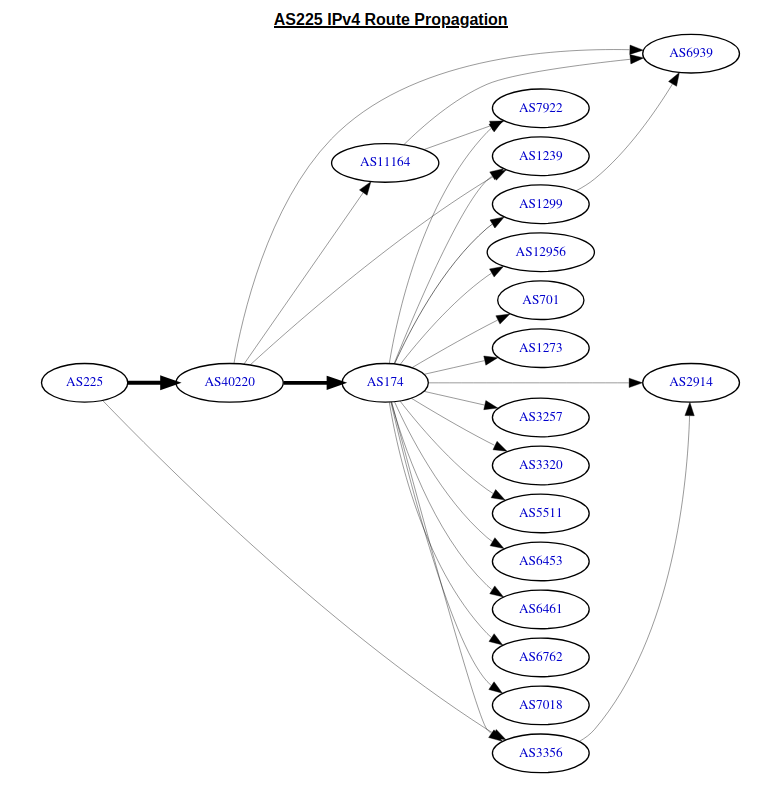
\includegraphics[width=0.5\textwidth]{../routing/as225-graph}
\end{frame}

\begin{frame}{AS40220}
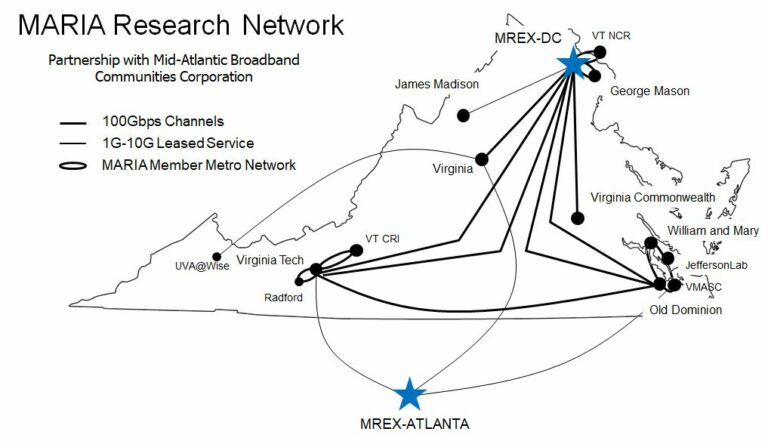
\includegraphics[height=0.8\textheight]{../routing/MARIA-Network-BW-768x441.jpg}
\end{frame}

\begin{frame}{}
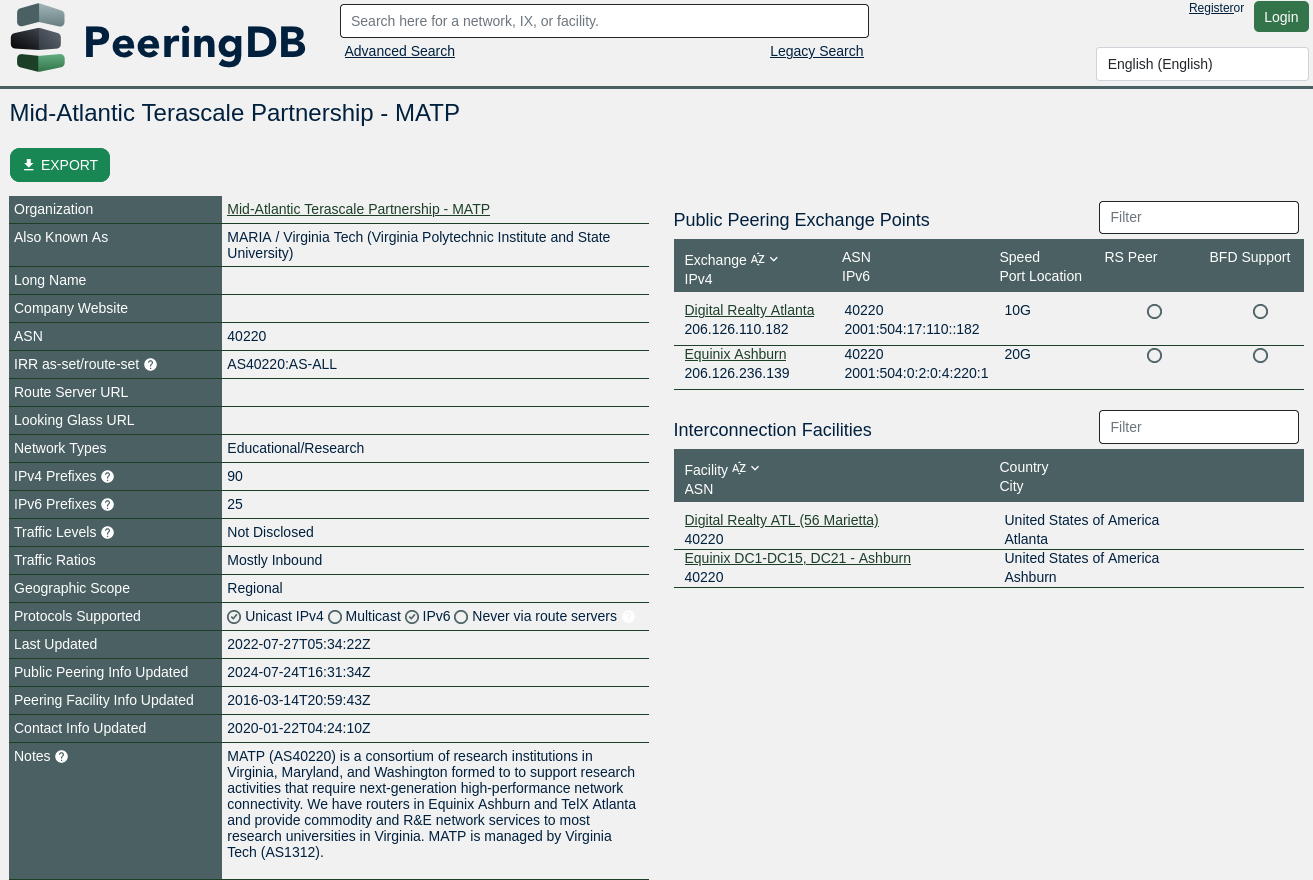
\includegraphics[width=0.95\textwidth]{../routing/as40220-peeringdb}
\end{frame}

\begin{frame}{AS3356}
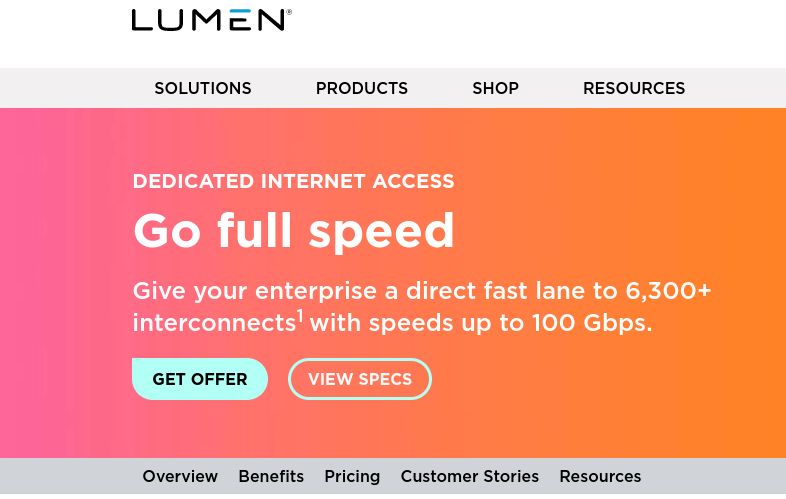
\includegraphics[height=0.8\textheight]{../routing/lumen-webpage.png}
\end{frame}

\begin{frame}{2024: AS3356 is a backup (8x prepend)}
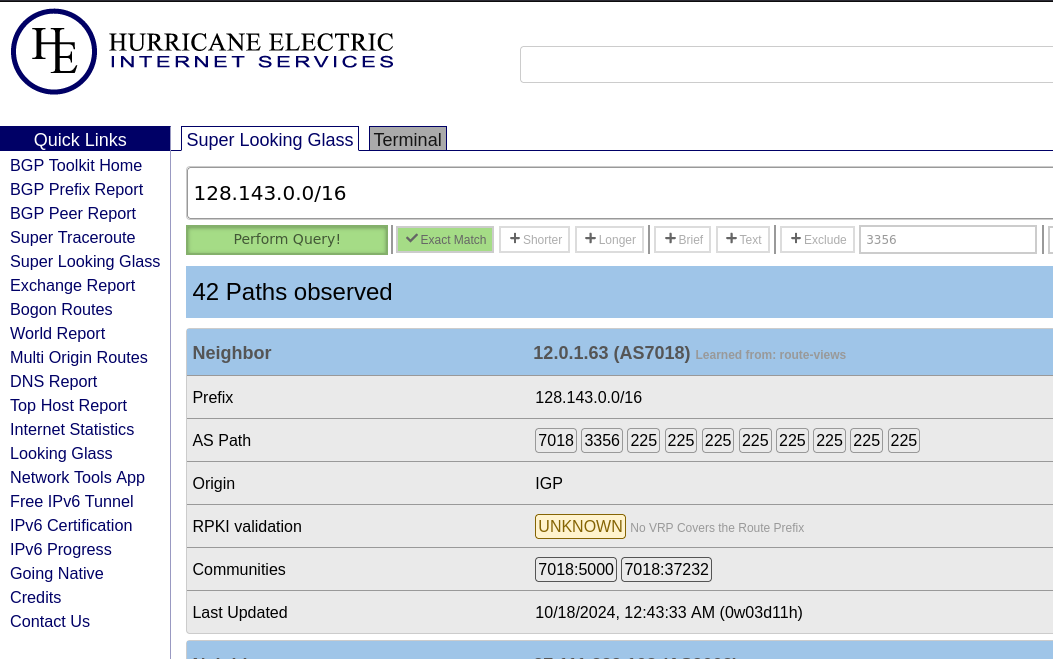
\includegraphics[height=0.8\textheight]{../routing/as3356-he-superlg.png}
\end{frame}

\begin{frame}
\frametitle{2025: AS3356 and AS 40220 equal?}
\includegraphics[height=0.8\textheight]{../routing/as3356-he-superlg-b.png}
\end{frame}
